\documentclass{beamer}
\usetheme{metropolis}
\usepackage{graphicx}
\usepackage{amsmath}
\usepackage{tcolorbox}
\title{Digital Signal Processing: COSC390}
\author{Jordan Hanson}
\institute{Whittier College Department of Physics and Astronomy}

\begin{document}
\maketitle

\begin{frame}{Unit 2.2 Outline}
\begin{enumerate}
\item Types of filters (reading: ch. 3, ch. 5)
\begin{itemize}
\item Butterworth
\item Bessel
\item Chebyshev
\end{itemize}
\item LTI systems and their properties (reading: ch. 5)
\item Convolution (reading: ch. 7)
\begin{itemize}
\item Implementation with FFT
\item Impulse and step response
\end{itemize}
\end{enumerate}
\textbf{These lectures will cover:} (Reading: chapter 19)
\begin{enumerate}
\item \textbf{Common filter kernels: Moving Average}
\item \textbf{General Recursive Filters: HP, LP, and Notch Examples}
\item \textbf{FIR and IIR definitions}
\end{enumerate}
\end{frame}

\section{Common filter kernels: Moving Average}

\begin{frame}{Common filter kernels: Moving Average}
The out of an LTI system such as a filter man be expressed as a \textit{convolution} of the transfer function coefficients $a_k$ and the data $x$. If the output is $y$, we may write
\begin{equation}
y[n] = \sum_{k=0}^{N-1} a_k x[n-k]
\end{equation}
\begin{figure}
\centering
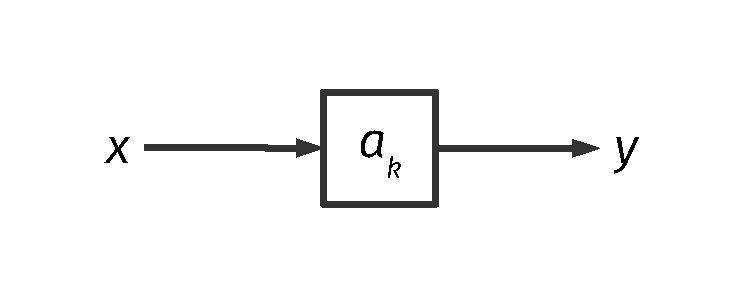
\includegraphics[width=0.6\textwidth]{figures/kernel1.pdf}
\caption{\label{fig:kernel1} A simple model for convolution as an LTI response.}
\end{figure}
\end{frame}

\begin{frame}{Common filter kernels: Moving Average}
The out of an LTI system such as a filter man be expressed as a \textit{convolution} of the transfer function coefficients $a_k$ and the data $x$. If the output is $y$, we may write
\begin{equation}
y[n] = \sum_{k=0}^{N-1} a_k x[n-k] + \sum_{k=0}^{N-1} b_k y[n-k]
\end{equation}
\begin{figure}
\centering
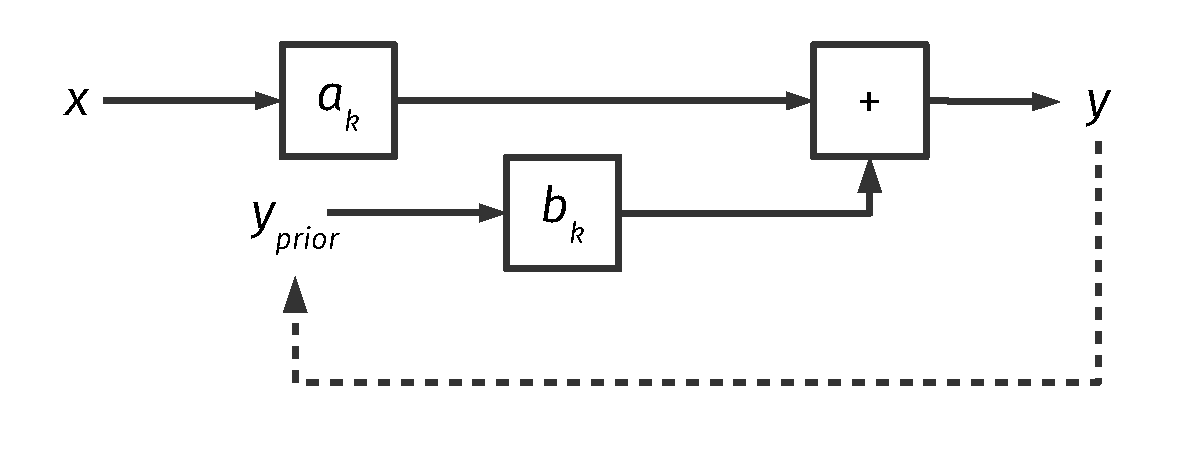
\includegraphics[width=0.75\textwidth]{figures/kernel2.pdf}
\caption{\label{fig:kernel2} A more general model for convolution as an LTI response.  These are the $a$ and $b$ coefficients of the octave \textit{filter} function.}
\end{figure}
\end{frame}

\begin{frame}[fragile]{Common filter kernels: Moving Average}
\textbf{Moving average filter with window-length $n$:}
\begin{enumerate}
\item $a_k$ are all equal to $1/n$
\item $b_k$ are zero
\end{enumerate}
Example:
\begin{itemize}
\item window-3 moving average: $a_0 = \frac{1}{3}$, $a_1 = \frac{1}{3}$, $a_2 = \frac{1}{3}$
\end{itemize}
\begin{verbatim}
y = filter(ones(window,1)/window,1,y);
\end{verbatim}
The filter function is expecting the $a_k$ and $b_k$ coefficients\footnote{For maximum confusion: the textbook and Octave use opposite conventions for $a_k$ and $b_k$.}.
\end{frame}

\section{Octave Programming Exercise: Moving Average}

\begin{frame}[fragile]{Common filter kernels: Moving Average}
Download the code \textbf{movingAverage.m} from Moodle, and run it at your desk.
\begin{enumerate}
\item What is happening to the spectrum?
\item Change the window parameter to various values.  What further changes do you observe in the noise and the spectrum?
\item What function shape do you observe in the spectrum with sufficient window size?
\end{enumerate}
\end{frame}

\begin{frame}{Common filter kernels: Moving Average}
\small
\begin{figure}
\centering
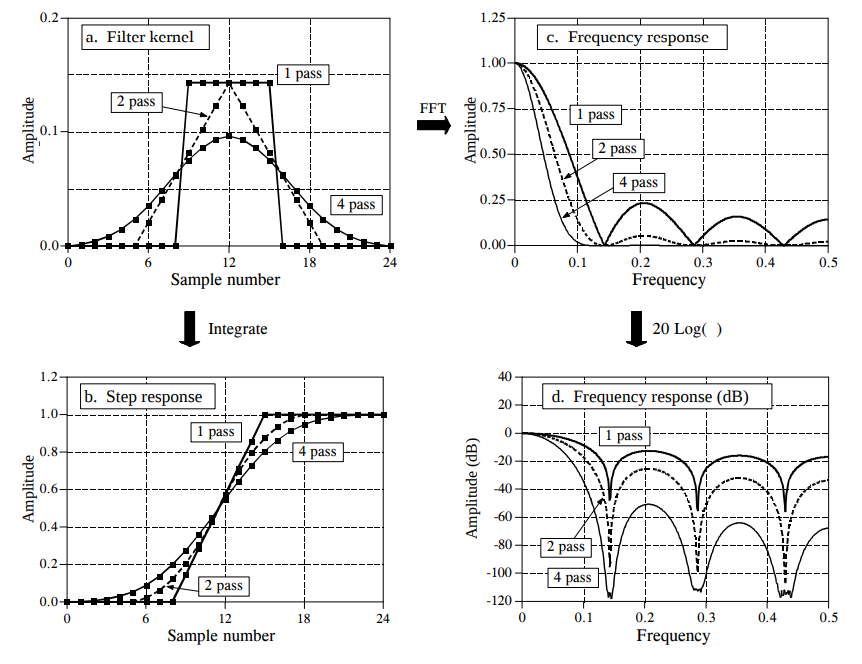
\includegraphics[width=0.7\textwidth]{figures/moving1.png}
\caption{\label{fig:moving1} Various effects of the moving average filter kernel. The moving average efficiently filters high-frequency noise in the time-domain.}
\end{figure}
\end{frame}

\begin{frame}{Common filter kernels: Moving Average}
\small
\begin{figure}
\centering
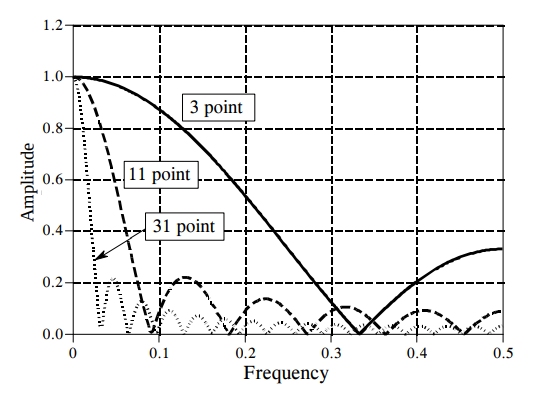
\includegraphics[width=0.7\textwidth]{figures/moving2.png}
\caption{\label{fig:moving2} The frequency response of a moving average filter is a \textit{sync}.  Why? (Calculations on board of filter kernel).}
\end{figure}
\end{frame}

\begin{frame}{Common filter kernels: Moving Average}
Frequency response of moving average filter, n-window:
\begin{equation}
h(f) = \frac{\sin(\pi f n)}{n\sin(\pi f)}
\end{equation}
\begin{itemize}
\item Basically, a sync
\item Modified by n-window instead of period
\end{itemize}
\end{frame}

\begin{frame}{Common filter kernels: Moving Average}
\small
\begin{figure}
\centering
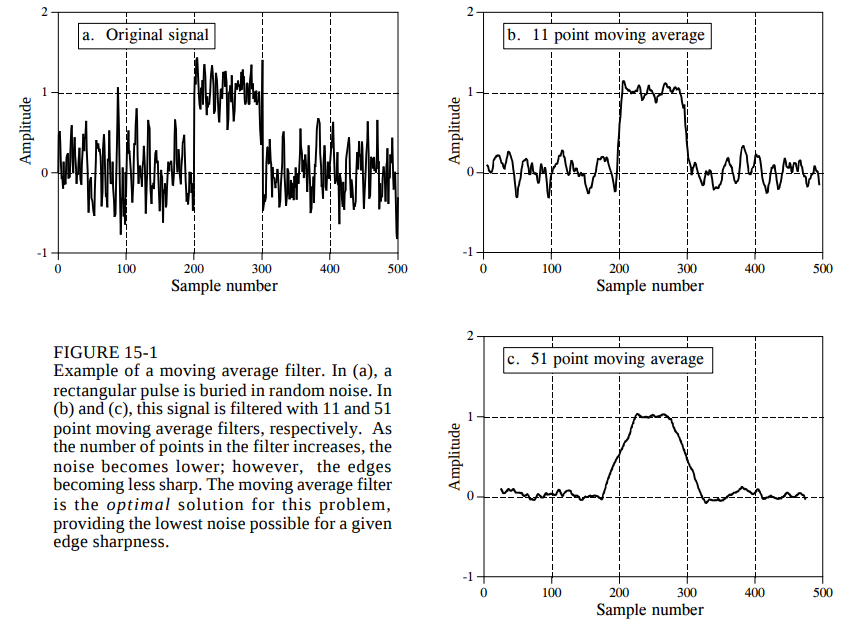
\includegraphics[width=0.7\textwidth]{figures/moving3.png}
\caption{\label{fig:moving3} The moving averege filter removes noise optimally while preserving step response.}
\end{figure}
\end{frame}

\section{Octave Programming Exercise: Finding the Signal}

\begin{frame}[fragile]{Finding the Signal}
Download the code \textbf{movingAverage2.m} from Moodle, and run it at your desk.
\begin{enumerate}
\item By tuning the moving average filter, can you reveal the signal?
\item Bonus: using older code, can you \textit{play this signal as audio} for varying window sizes?
\end{enumerate}
\end{frame}

\section{Octave Programming Exercise: Single-Pole Recursion Formulas}

\begin{frame}[fragile]{Single-Pole Recursion Formulas}
\textbf{Single-pole LP filter recursion:}
\begin{enumerate}
\item $a_0 = 1-x$
\item $b_1 = x$
\end{enumerate}
The variable $x$ varies from $[0,1]$.  It is the amount of decay between samples:
\begin{equation}
x = \exp(-1/d)
\end{equation}
The $x$ parameter is related to the cutoff-frequency:
\begin{equation}
x = \exp(-2\pi f_c)
\end{equation}
\textbf{Exercise:} implement this in movingAverage2.m and recover the signal with the single-pole LP filter.  Note: we are not using the \textbf{butter} function...How would you achieve the effect of multiple poles?
\end{frame}

\begin{frame}[fragile]{Single-Pole Recursion Formulas}
\textbf{Single-pole HP filter recursion:}
\begin{enumerate}
\item $a_0 = (1+x)/2$
\item $a_1 = -(1+x)/2)$
\item $b_1 = x$
\end{enumerate}
The variable $x$ varies from $[0,1]$.  It is the amount of decay between samples:
\begin{equation}
x = \exp(-1/d)
\end{equation}
The $x$ parameter is related to the cutoff-frequency:
\begin{equation}
x = \exp(-2\pi f_c)
\end{equation}
\textbf{Exercise:} implement this in movingAverage2.m and recover the signal with the single-pole HP+LP filter.
\end{frame}

\section{Octave Programming Exercise: Notch and Narrow band-pass}

\begin{frame}[fragile]{Notch and Narrow band-pass}
\small
\textbf{Implement the following recursive formula, and see what it does to noise\footnote{It's probably best to recycle code from movingAverage.m to a new file.}:}
\begin{enumerate}
\item $a_0 = 1-K$
\item $a_1 = 2(K-R)\cos(2\pi f)$
\item $a_2 = R^2-K$
\item $b_1 = 2R\cos(2\pi f)$
\item $b_2 = -R^2$
\end{enumerate}
($R = 1-3 BW$, where $BW$ is the bandwidth, centered on the frequency $f$).  For K, we have
\begin{equation}
K = \frac{1-2R\cos(2\pi f)+R^2}{2-2\cos(2\pi f)}
\end{equation}
\end{frame}

\begin{frame}[fragile]{Notch and Narrow band-pass}
\small
\textbf{Implement the following recursive formula, and see what it does to noise\footnote{It's probably best to recycle code from movingAverage.m to a new file.}:}
\begin{enumerate}
\item $a_0 = K$
\item $a_1 = -2K\cos(2\pi f)$
\item $a_2 = K$
\item $b_1 = 2R\cos(2\pi f)$
\item $b_2 = -R^2$
\end{enumerate}
($R = 1-3 BW$, where $BW$ is the bandwidth, centered on the frequency $f$).
\end{frame}

\begin{frame}[fragile]{Notch and Narrow band-pass}
\begin{enumerate}
\item Add a sine-tone to your noise sample, and then isolate it with the band-pass filter.
\item Now make the noise small, but add several other \textit{unwanted sine-tones} to the data, and filter them out with the band-reject.
\end{enumerate}
So now we start to see how simple it is to clean the data of unwanted noise and signals, using only recursive relationships between input and output data!  However, we must eventually make a distinction between \textbf{FIR and IIR.}
\end{frame}

\section{Theory and Examples: Phase Response}

\begin{frame}{Phase Response}
\small
\begin{figure}
\centering
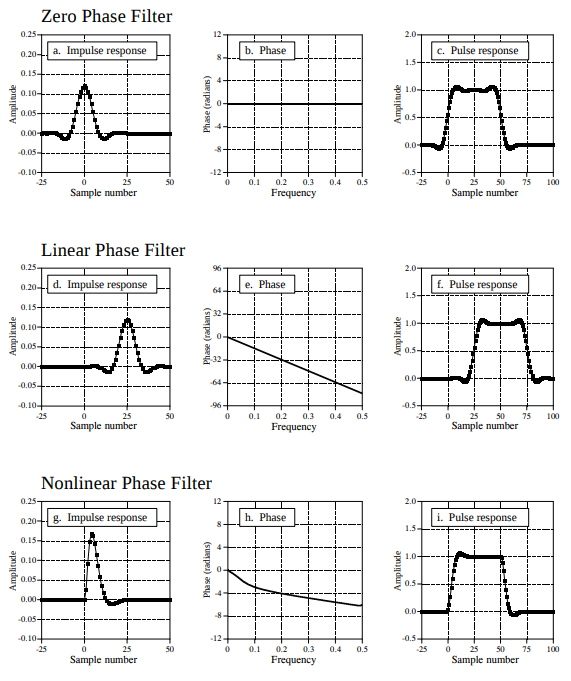
\includegraphics[width=0.5\textwidth]{figures/phase.png}
\caption{\label{fig:phase} The problem with many filters is that they introduce non-zero or non-linear phase response.  How do we eliminate this?}
\end{figure}
\end{frame}

\begin{frame}{Phase Response}
\begin{enumerate}
\item Review \textbf{group delay:} $\tau_g = - \frac{d\phi}{d\omega}$.
\item Discuss \textit{unwrapping} if necessary.
\item Changing zero group delay to linear (time-shift, causality).
\item Taking $t \rightarrow -t$? What phase shift does this cause?  What is the total group delay?
\end{enumerate}
\end{frame}

\end{document}
